\documentclass[10pt,a4paper,twocolumn]{ctexart}

\usepackage[margin=2cm,columnsep=0.75cm]{geometry}
\usepackage{booktabs}
\usepackage{graphicx}
\usepackage{caption}
\usepackage{amsmath}
\usepackage{balance}
\usepackage{float}

\pagestyle{plain}

\setmainfont{TeX Gyre Pagella}
\setsansfont{TeX Gyre Heros}
\setCJKmainfont{Noto Serif CJK SC}
\setCJKsansfont{Noto Sans CJK SC}

\captionsetup{font=small,labelfont=bf}
\ctexset{
  section = {format = \sffamily\bfseries\large},
  subsection = {format = \sffamily\bfseries\normalsize},
}
\renewcommand{\refname}{参考文献}

\newcommand{\NumSamples}{188}
\newcommand{\NumCorrect}{180}
\newcommand{\AccTotal}{95.7\%}
\newcommand{\AccCILow}{91.8\%}
\newcommand{\AccCIHigh}{97.8\%}
\newcommand{\InputTokens}{122\thinspace404}
\newcommand{\OutputTokens}{8\thinspace460}
\newcommand{\TotalCost}{0.0051}
\newcommand{\NCertain}{134}
\newcommand{\PctCertain}{71.3\%}
\newcommand{\AccCertain}{99.3\%}
\newcommand{\NUncertain}{54}
\newcommand{\AccUncertain}{87.0\%}
\newcommand{\MeanProbCorrect}{0.99}
\newcommand{\MeanProbWrong}{0.83}
\newcommand{\NWrong}{8}
\newcommand{\LowBinN}{7}
\newcommand{\LowBinCorrect}{4}
\newcommand{\LowBinAcc}{57.1\%}
\newcommand{\ModelLetterA}{48}
\newcommand{\ModelLetterB}{41}
\newcommand{\ModelLetterC}{53}
\newcommand{\ModelLetterD}{46}
\newcommand{\KeyLetterA}{47}
\newcommand{\KeyLetterB}{42}
\newcommand{\KeyLetterC}{51}
\newcommand{\KeyLetterD}{48}


\title{\sffamily JEV-1.13 高中美国历史测试报告}
\author{}
\date{2026 年 9 月 28 日}

\begin{document}
\maketitle

\section*{摘要}
本报告记录模型 JEV-1.13 在 MMLU 基准高中美国历史科目上的测试结果。测试共
\NumSamples{} 道四选一单选题，模型答对 \NumCorrect{} 道，准确率
\AccTotal{}，远高于 25\% 的随机水平。模型为每题给出各选项的概率，其中所选选项的概率下称所选概率：该概率为
1.00 的 \NCertain{} 题几乎全对（\AccCertain{}），低于 1.00 的
\NUncertain{} 题准确率为 \AccUncertain{}。整次测试消耗输入 \InputTokens{}
token、输出 \OutputTokens{} token，总费用 \TotalCost{} 美元。在该场景下，模型答题准确、代价极低，其给出的概率能标示答案的可靠程度。

\section{数据集}
数据来自 MMLU（Massive Multitask Language Understanding）基准的高中美国历史科目测试集~\cite{mmlu}。测试共
\NumSamples{} 题，均为四选一单选题。每题由一段材料（文献引文或情境描述）和一个设问构成，模型需选出唯一正确选项。标准答案由数据集提供，在四个选项字母上的分布接近均匀（A
\KeyLetterA{} 题、B \KeyLetterB{} 题、C \KeyLetterC{} 题、D \KeyLetterD{}
题）。被测对象为模型 JEV-1.13（标识 \texttt{typesafe/jev-1.13-20260917}）。

\section{结果}
以下结果均以数据集提供的标准答案为判据。

\subsection{整体结果}
表~\ref{tab:overall} 给出整体结果。\NumSamples{} 题中模型答对
\NumCorrect{} 题，准确率 \AccTotal{}（95\% 置信区间
\AccCILow{}--\AccCIHigh{}）。四选一题随机猜测的期望准确率为
25\%，模型的成绩远高于该水平。

\begin{table}[htbp]
  \centering
  \caption{整体结果}
  \label{tab:overall}
  \begin{tabular}{lc}
    \toprule
    项目 & 数值 \\
    \midrule
    题目数 & \NumSamples \\
    答对题数 & \NumCorrect \\
    准确率 & \AccTotal \\
    95\% 置信区间 & \AccCILow{}--\AccCIHigh \\
    \bottomrule
  \end{tabular}
\end{table}

\subsection{所选概率与准确率}
除所选答案外，模型还给出每题四个选项各自的概率；取其中所选选项的概率，记为所选概率。

\NCertain{} 题（\PctCertain{}）的所选概率为 1.00，其中 \AccCertain{}
答对；其余 \NUncertain{} 题低于 1.00，准确率为 \AccUncertain{}。\NumCorrect{}
道答对题的平均所选概率为
\MeanProbCorrect{}，\NWrong{} 道答错题的平均所选概率为 \MeanProbWrong{}。

图~\ref{fig:prob} 按所选概率分档给出题目数与准确率。低于 0.90 的
\LowBinN{} 题中仅 \LowBinCorrect{} 题答对；各档准确率随所选概率总体上升，0.99
档与 1.00 档均超过 99\%。所选概率能区分答案的可靠程度，可作为判断单题答案可信与否的参考。

\begin{figure}[htbp]
  \centering
  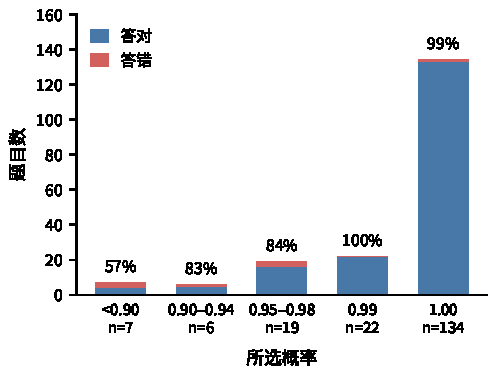
\includegraphics[width=\columnwidth]{figures/fig_prob_zh.pdf}
  \caption{按所选概率分档的题目数与准确率。柱高为该档题目数，蓝色为答对、红色为答错，柱顶百分比为该档准确率。}
  \label{fig:prob}
\end{figure}

\subsection{调用成本}
如表~\ref{tab:cost} 所示，整次测试消耗输入 \InputTokens{} token、输出
\OutputTokens{} token，总费用 \TotalCost{} 美元。

\begin{table}[H]
  \centering
  \caption{调用成本}
  \label{tab:cost}
  \begin{tabular}{lc}
    \toprule
    项目 & 数量 \\
    \midrule
    输入 token & \InputTokens \\
    输出 token & \OutputTokens \\
    总费用 & \TotalCost{} 美元 \\
    \bottomrule
  \end{tabular}
\end{table}

\balance
\section{结论}
在 \NumSamples{} 道高中美国历史四选一题上，JEV-1.13 答对 \NumCorrect{}
道，准确率 \AccTotal{}，远高于随机水平；七成以上的题所选概率为
1.00，且几乎全对，而所选概率低于 0.90 的题不足六成答对。整次测试总费用约半美分。综合看，JEV-1.13
在该场景下答题准确、代价极低，其给出的所选概率可用于识别不可靠的答案。

\begin{thebibliography}{9}
\bibitem{mmlu}
Dan Hendrycks, Collin Burns, Steven Basart, Andrew Critch, Jerry Li, Dawn
Song, Jacob Steinhardt.
\emph{Measuring Massive Multitask Understanding}.
ICLR 2021. 数据取自 \texttt{cais/mmlu} 测试集。
\end{thebibliography}

\end{document}
